%!TEX root = master.tex

\section{\$ java -history}



\begin{frame}
  \frametitle{\$ java -history}
  \begin{itemize}
    \item Created by James Gosling in 1995 (Sun Microsystems, later Oracle)
    \begin{center}
      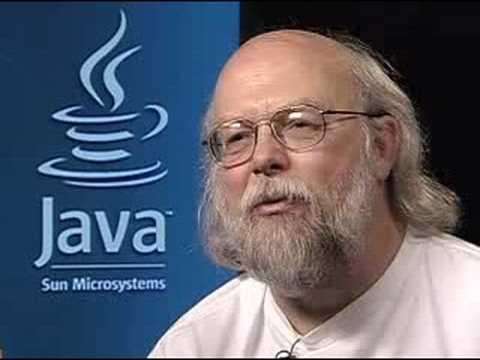
\includegraphics[width=0.5\textwidth]{fig/old}
      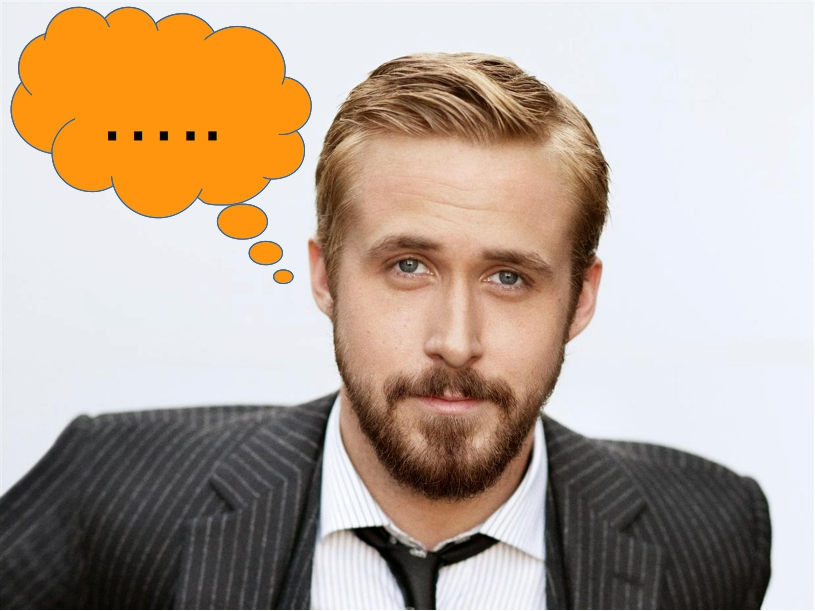
\includegraphics[width=0.5\textwidth]{fig/young}
    \end{center}

    \item Typing: strong (no implicit casting, mostly), static (variables have types)
    \item Cross-platform (kind of...)
    \item Paradigms: object-oriented, structured, imperative, functional, generic, reflective, concurrent
  \end{itemize}
\end{frame}



